\chapter{Testing}

\section{Overall Approach to Testing}

This chapter presents a multitude of different testing types. There are authomated unit tests to ensure the internal code logic behaves as expected. The User Interface tests are tests which are difficutly to automate but are used to esnure that the user interface encaptures the correct state of execition. Stress testing is deployed to test the applications robustness. Finally acceptance testing is used to assess how well the applications meets the specified requirements in section \ref{funcymcdunky}.

\section{Unit Tests}

Unit tests were developed using the JUnit framework and have been designed by the author to test a series of boundary conditions and any underlying algorithmic logic present with the application code. The execution of these tests than then be fully automated and using the built in interface provided by Eclipse a summary of the completed tests can be viewed by the author enabling clear identification of failed tests and reason for failure. The unit tests are generally only performed on the Model package. The view package is difficult to unit test as it requires user input and is therefore manually tested by the author. The controller package does not really contain any behaviour worthy of testing as it mainly consists of simple assignments or the calling of other system functions.

There are features present in the application code which the author has excluded from the unit testing process. Any feature which relies on random numbers to perform its task has not been unit tested. As a random number is used the author feels that they cant reliably be tested, therefore it doesn’t makes sense to attempt to. Instead the author has extracted the code which relies on such random numbers and tested the behaviour of such code using specifically defined values, this enables the author to accurately test for expected behaviours. In addition to this getter and setter methods or simple assignment operations have not been tested. The reason for excluded these methods from unit tests is because the code responsible is so simple it can’t fail so there is no real purpose in producing such tests.

The unit tests that the author has produced revolve around ensuring that only legal algorithm parameters are accepted and that the movement, probability and pheromone functions are behaving as expected and return legal values. These tests contain validation checks against a range of values for each parameter including boundary conditions to ensure that they are correctly dealt with, examples of such testing can be seen in figures \ref{testAlpha} - \ref{testAgent}. The probability and pheromone functions are tested to ensure the correct value is returned and in the case of probability, ensure that the sum of all calculated probabilities is equal to 1, such a test is shown in figure \ref{testProb}. There are many more tests present in the test package for the application however the author has only briefly outlined a small number of these, evidence of such testing can be seen below in figure \ref{testSS}.

\begin{figure}[H]
\centering
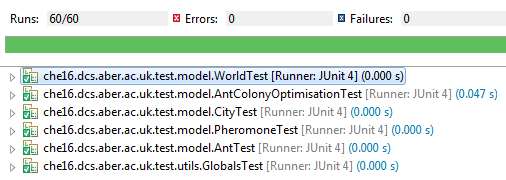
\includegraphics[scale=0.8]{Images/chapter6/testSS}
\caption{Evidence of the completed execution of the applications unit tests. The view present is the built in Eclipse JUnit interface.}
\label{testSS}
\end{figure}

\section{User Interface Testing}

\section{Stress Testing}

\section{Acceptance}

\section{User Testing}

Detailed descriptions of every test case are definitely not what is required here. What is important is to show that you adopted a sensible strategy that was, in principle, capable of testing the system adequately even if you did not have the time to test the system fully.

Have you tested your system on �real users�? For example, if your system is supposed to solve a problem for a business, then it would be appropriate to present your approach to involve the users in the testing process and to record the results that you obtained. Depending on the level of detail, it is likely that you would put any detailed results in an appendix.

The following sections indicate some areas you might include. Other sections may be more appropriate to your project. 